\laborator{Определение условий фазовых равновесий пар~-- жидкость}

\goal на основе экспериментальных данных по давлению насыщенных паров чистых компонентов определить условия фазовых равновесий пар~-- жидкость бинарной идеальной смеси при различных термодинамических условиях; результаты представить в виде диаграмм фазового равновесия ($у-х$; $Р-х, у$; $Т-х, у$).

\subsubsection{Теория}

Химической промышленности в основном приходится иметь дело с системами, представляющими собой смеси газов и жидкостей, которые необходимо разделять. При проектировании процессов разделения подобных систем необходимо иметь данные о равновесных свойствах смесей. Условия фазового равновесия удобно представлять в виде фазовой диаграммы, которая описывает влияние температуры, давления и состава на вид и число фаз, которые могут сосуществовать при данных условиях. Число фаз определяется согласно правилу фаз Гиббса. Вид фаз, которые могут сосуществовать в конкретных условиях, зависит от химической природы компонентов. Представление фазового равновесия более удобно в графическом виде, чем в табличном, так как позволяет охватить взаимные связи между переменными.

В соответствии с правилом фаз Гиббса для любой термодинамически равновесной системы число параметров состояния $С$ (степеней свободы), которые можно изменять, сохраняя число существующих фаз $Ф$ неизмененным, определяется выражением
\begin{equation}
С=К-Ф+N,
\end{equation}
где $К$ – число компонентов системы, $N$ – число параметров состояния системы, имеющих одно и то же значение во всех фазах (обычно температура $Т$ и давление $p$, $N$ = 2). Величина $С$ определяет число параметров состояния, которые нужно задать для однозначного определения состояния системы.

Из правила фаз следует, что в однокомпонентной системе ($К$ = 1) в однофазной области ($Ф$ = 1) состояние системы определяется двумя параметрами ($С$ = 2) $Т$ и $p$ (можно произвольно и одновременно изменять оба параметра до тех пор, пока система не окажется на одной из ограничивающих область линий). На линиях фазового равновесия ($Ф$ = 2) состояние системы определяется одним параметром ($С$ = 1) (произвольно можно менять только один из параметров – $p$ или $Т$ (если изменяется $Т$, то $p$ будет изменяться в соответствии с ходом кривой, и наоборот)). В трехфазной области ($Ф$ = 3) число степеней свободы равно нулю ($С$ = 0), что соответствует тройной точке (в этой точке ни один из параметров не может быть изменен, равновесное сосуществование трех фаз однокомпонентной системы возможно только при строго определенных значениях $Т$ и $p$.). Для любой системы число фаз максимально, когда $С$ = 0. При увеличении числа компонентов $К$ в системе растет число параметров состояния $С$, необходимых для однозначного определения состояния системы.

Как было показано выше, для однокомпонентной системы максимальное число степеней свободы равно двум, соответственно фазовое равновесие такой системы можно представить на плоскости в виде двухкоординатной фазовой диаграммы (\cref{fig:phase-id.f1}). Для двухкомпонентной системы число степеней свободы равно трем. Взаимозависимость трех переменных можно отразить лишь посредством пространственных диаграмм. На практике работать с трехмерными диаграммами уже сложнее, чем с двухмерными. Для трехкомпонентной системы число степеней свободы равно четырем и представить фазовую диаграмму такой системы графически уже затруднительно.

\begin{figure}
	\begin{center}
		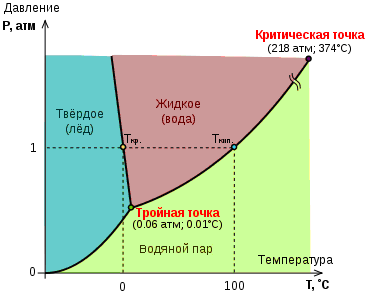
\includegraphics[width=0.7\textwidth]{phase-id-f1.png}
	\end{center}
	\caption{Двухкоординатная фазовая диаграмма воды} \label{fig:phase-id.f1}
\end{figure}

Однако возможен альтернативный подход, позволяющий упростить построение пространственных диаграмм. Например, в случае двухкомпонентной смеси можно использовать серию плоскостных диаграмм при фиксированном значении третьей переменной. Пример таких диаграмм показан на рисунке \cref{fig:phase-id.f2}, это плоскости Р1, Р2, Р3 и т.д.
\begin{figure}
	\begin{center}
		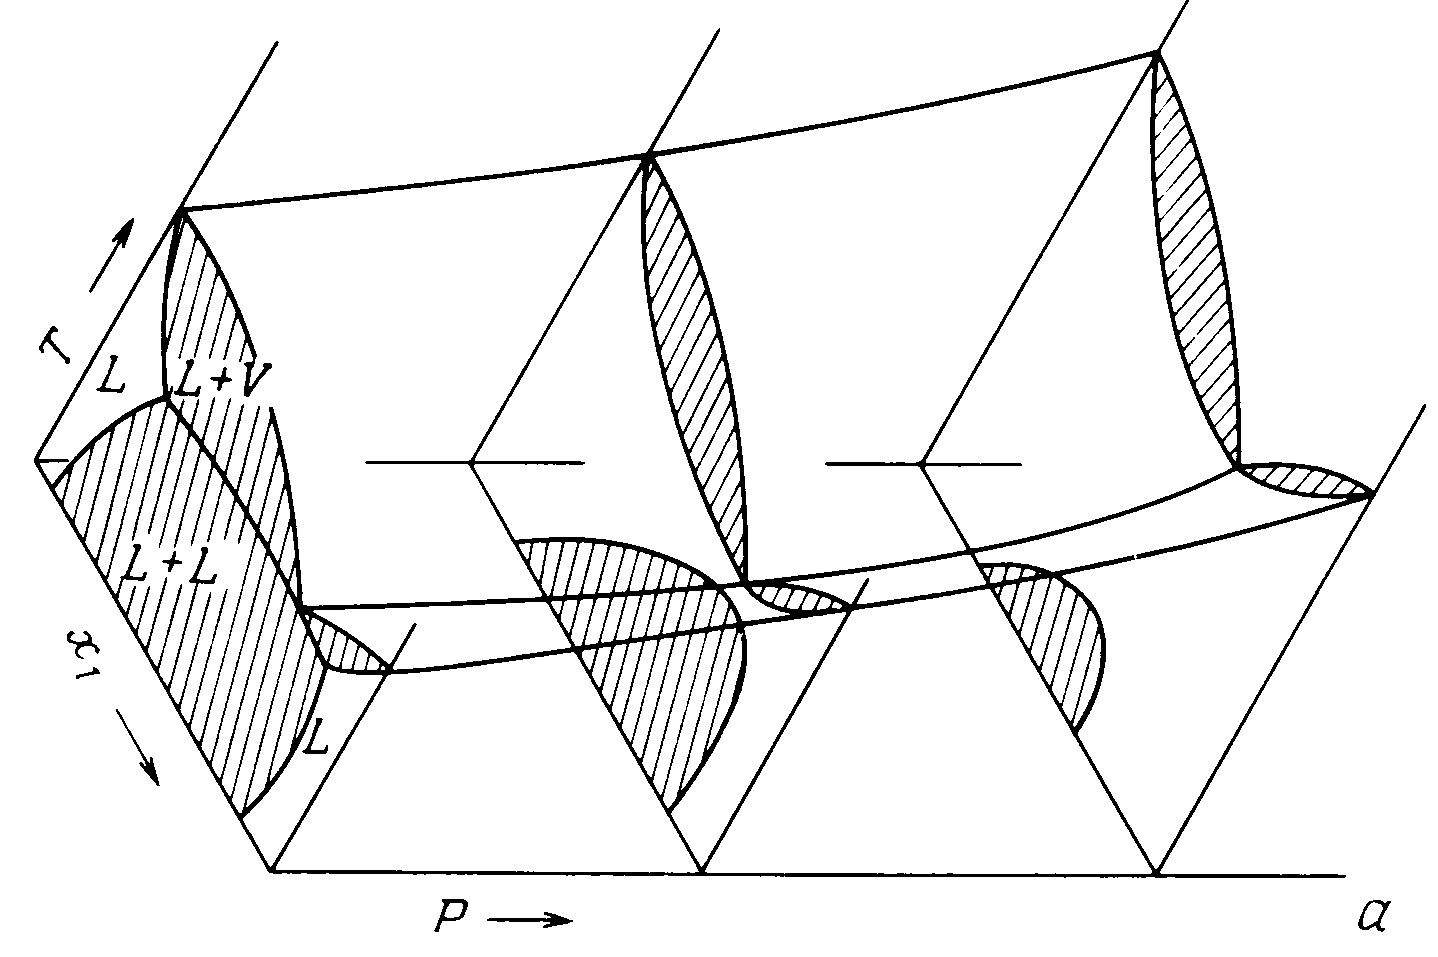
\includegraphics[width=0.8\textwidth]{phase-id-f2.png}
	\end{center}
	\caption{Трехмерная фазовая диаграмма бинарной смеси} \label{fig:phase-id.f2}
\end{figure}

Обычно используют следующие виды диаграмм:
\begin{itemize}
\item в виде изобарических сечений $(p = const)$, которые демонстрируют влияние $Т$ и общего состава смеси на состояние фаз системы (пример такой диаграммы для бинарной смеси представлен на рисунке \cref{fig:phase-id.f3}); 
\item в виде изотермических сечений $(Т = const)$, которые демонстрируют влияние $p$ и общего состава смеси на состояние фаз системы;
\item в виде изоплет (диаграммы постоянного состава), которые демонстрируют влияние $p$ и $Т$ на состояние фаз системы при постоянном составе смеси.	
\end{itemize} 

При построении диаграммы для удобства обычно ограничиваются показом отношений между определенным числом фаз, например пар~-- жидкость, жидкость~-- жидкость, жидкость~-- твердая фаза. Для решения практических задач необходимы лишь ограниченные области $Т$ и $p$, число рассматриваемых фаз также ограничено. При проектировании большинства процессов химической технологии наибольшей интерес представляет набор диаграмм для систем пар~-- жидкость. В этом случае, например диаграмма фазового равновесия (рисунок \cref{fig:phase-id.f3}) является избыточной, так как интерес представляет только ее верхняя часть, где представлена система пар~-- жидкость. 

\begin{figure}
	\begin{center}
		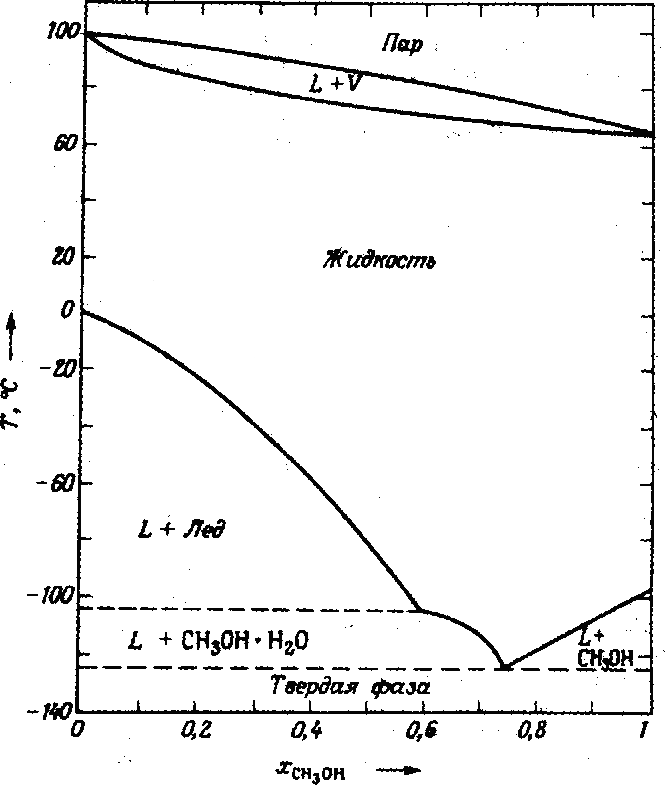
\includegraphics[width=0.5\textwidth]{phase-id-f3.png}
	\end{center}
	\caption{Диаграмма фазового равновесия (пар – жидкость – твердая фаза) в системе метанол + вода при $p = 0.1 МПа$} \label{fig:phase-id.f3}
\end{figure}

На рисунке \cref{fig:phase-id.f4} представлены основные типы фазовых диаграмм систем пар ~-- жидкость. Представленный вид диаграмм характерен для систем с плавным изменением температур кипения растворов в диапазоне температур между температурами кипения чистых жидкостей, включая системы, подчиняющиеся закону Рауля. Вид этих зависимостей определяется свойствами компонентов смеси. Например, для идеальной смеси зависимость $p-х$ при $T=const$ в соответствии с законом Рауля будет прямой линией.

\begin{figure}
	\begin{center}
		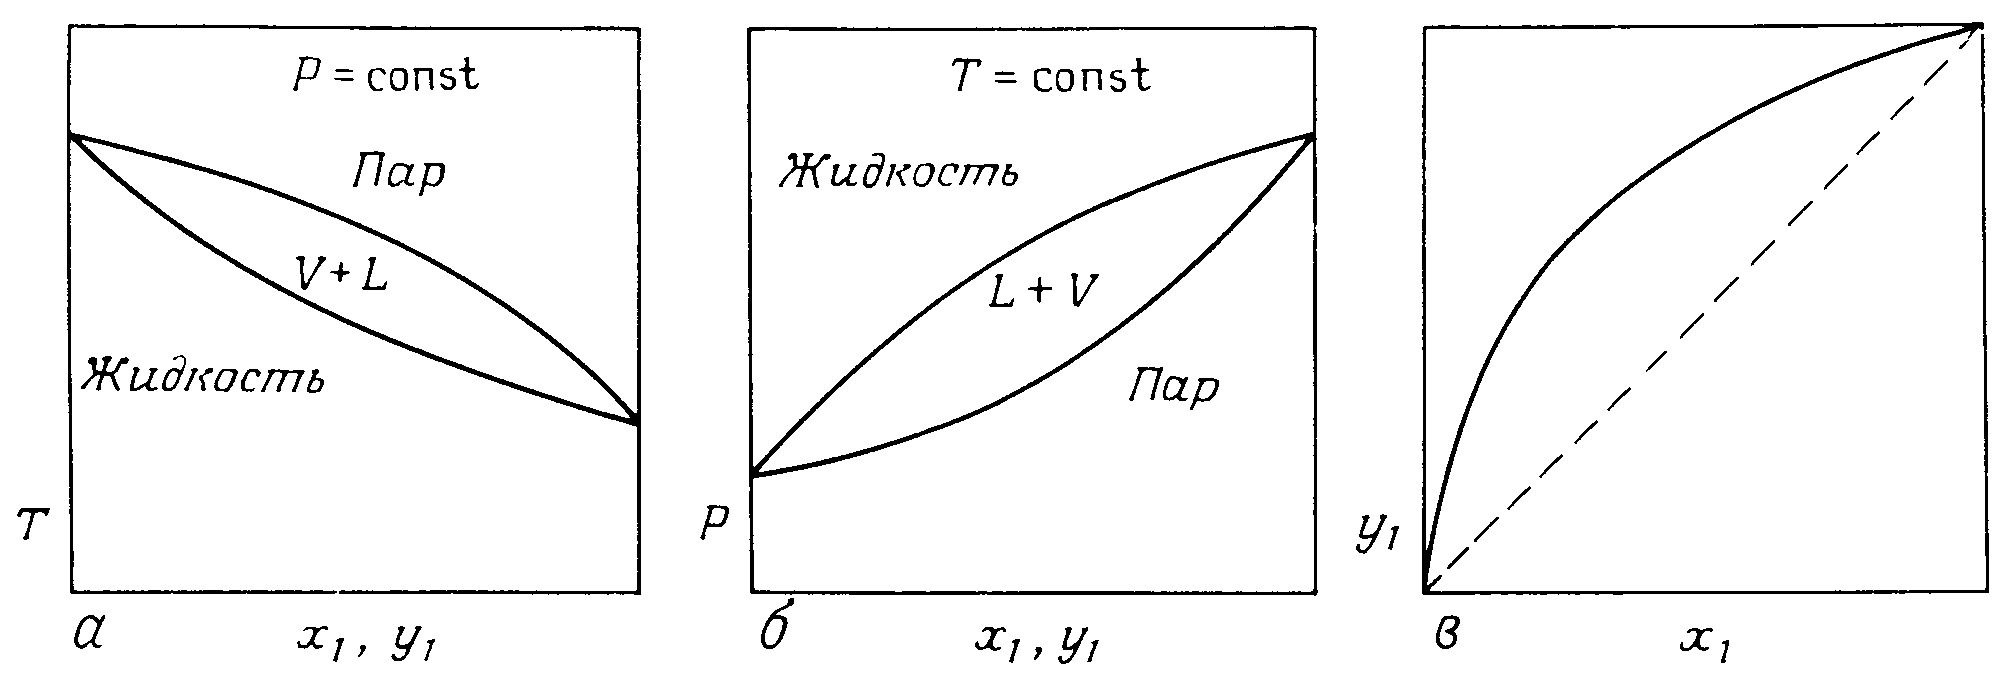
\includegraphics[width=0.9\textwidth]{phase-id-f4.png}
	\end{center}
	\caption{Двухкоординатные фазовые диаграммы $Т – х, у$ (а); $p – х, у$ (б); $х – y$ (в), показывающие паровую и жидкую фазы} \label{fig:phase-id.f4}
\end{figure}

Для технических расчетов наиболее важной является диаграмма $T-x, у$ --- зависимость температур кипения жидкости и конденсации паров от составов жидкой и паровой фаз, так как процессы перегонки в промышленных аппаратах протекают в изобарных условиях. Для проведения расчетов использование данных о фазовом равновесии в графическом виде не всегда удобно, особенно при решении задач оптимизации. В этой связи условия фазовых равновесий удобно представлять в виде системы уравнений, решение которой позволит определить искомые параметры равновесия. 



\subsubsection{Определение условий фазового равновесия}
Условия равновесия двух фаз $n$--компонентной системы при заданной температуре $T$ определяются следующей системой уравнений:
\begin{equation}\label{eq:phas.equi}
\left\lbrace 
\begin{gathered} 
T^{I}=T^{II},\\
p^{I}(T,x_1,x_2,...,x_n-1)=p^{II}(T,y_1,y_2,...,y_n-1),\\
\mu_i^{I}(T,x_1,x_2,...,x_n-1)=\mu^{II}_i(T,y_1,y_2,...,y_n-1),
\end{gathered} 
\right.
\end{equation}
где $\mu$ --- химический потенциал (верхний индекс обозначает фазу, нижний – компонент). Чтобы определить условия фазового равновесия, необходимо решить систему уравнений \eqref{eq:phas.equi}. Численное решение данной системы можно получить, если выражения для химического потенциала и давления представлены в явном виде.
В однокомпонентном случае химический потенциал определяется следующим образом:
\begin{equation}
\int\limits_{\mu^0}^{\mu} d \mu=\dfrac{1}{N} \int\limits_{p^0}^{p} Vdp.
\end{equation}

Отсюда можно получить явный вид для химического потенциала, однако это возможно только если известно уравнение состояния. В случае использования уравнения состояния идеального газа $pV=NRT$ выражение будет иметь вид:
\begin{equation} \label{eq:phase.muid}
	\mu(T,p)=\mu^0(T)+RT \ln (p),
\end{equation}
где $\mu^0(T)$ --- химический потенциал идеального газа при единичном давлении. В случае смеси выражение \eqref{eq:phase.muid} будет иметь следующий вид:
\begin{equation} \label{eq:phase.muidi}
	\mu_i (T,p,x) = \mu_i^0(T) + RT \ln(p_i),
\end{equation}
где $p_i=p x_i$ --- парциальное давление компонента $i$ в смеси.

Для систем, не подчиняющихся уравнению идеального газа вводится понятие летучести (фугитивности): $f=p \gamma_f$ ($f_i=p_i \gamma_{f_i}$), где $\gamma_f$ --- коэффициент летучести (фугитивности), который зависит от $T$, $p$ и состава в случае смеси. Выражение химического потенциала в этом случае запишется следующим образом:
\begin{equation} \label{eq:phase.mureal}
	\mu_i (T,p,x) = \mu_i^0(T) + RT \ln(f_i).
\end{equation}
В случае идеального газа $\gamma_f=1$.
Выражения \cref{eq:phase.muid,eq:phase.muidi,eq:phase.mureal} записаны в случае, когда в качестве системы отсчета для химического потенциала выбрано состояние идеального газа $\mu^0(T)$, что не всегда удобно. Кроме того, коэффициент летучести (фугитивности) может быть определен, только если известно уравнение состояния реального вещества. 

В качестве системы отсчета для жидких смесей часто выбирают химический потенциал чистой жидкости  при тех же $p$ и $T$, что и раствор. В этом случае выражение химического потенциала для жидкой смеси запишется в виде:
\begin{equation}
	\mu_i(T,p,x)=\mu_i^0(T,p)+R T \ln (a_i),
\end{equation}
где $а_i$ --- активность, величина, учитывающая концентрационную зависимость химического потенциала компонентов реального раствора:
\begin{equation}
	a_i=\gamma_i x_i,
\end{equation}
где $\gamma_i$ --- коэффициент активности компонента $i$, в случае идеального раствора $\gamma_i =1 $.

Необходимо отметить, что стандартная часть химического потенциала (первое слагаемое) не зависит от концентрации (см. уравнения \cref{eq:phase.muid,eq:phase.muidi,eq:phase.mureal} ), концентрационная зависимость учитывается вторым слагаемым.

Теперь первое уравнение условий фазового равновесия пар~-- жидкость \eqref{eq:phas.equi} можно записать в виде:
\begin{equation}
	\mu_i^0(T)+RT \ln (f_i)=\mu_i^0(T,p)+ R T \ln (a_i),
\end{equation}
откуда после преобразований можно получить следующее выражение, связывающее концентрации в фазах:
\begin{equation} \label{eq:phase.yreal}
	y_i=\dfrac{f_i^0 \gamma_i x_i}{\gamma_{f_i} p},
\end{equation}
где $f_i^0$ --- летучесть (фугитивность) чистого компонента $i$ при заданных $Т$ и $p$. 
По правилу фаз Гиббса двухфазная система имеет $n$ степеней свободы:
\begin{equation*}
	С=К-Ф+2=n-2+2=n.
\end{equation*}

Для $n$ независимых параметров, полностью определяющих состояние системы, обычно выбирают $n-1$ концентраций в жидкой фазе и $p$ или $Т$.

Следовательно, для определения состава паровой	 фазы и $p$ достаточно системы, состоящей из $n$ уравнений вида \eqref{eq:phase.yreal}, определяющих концентрации в паровой фазе, дополненной выражением
\begin{equation}
	\sum\limits_{i=1}^{n} y_i =1.
\end{equation}

Данная система уравнений может быть упрощена, если принять, что:
\begin{itemize}
	\item паровая фаза подчиняется  уравнению состояния идеального газа, т.е. ${\gamma_f}_i$;
	\item при небольших давлениях значение летучести близко к давлению насыщенных паров чистого компонента $f_i^0 \approx p^0_i (T)$.
\end{itemize}
В итоге получим:
\begin{equation} \label{eq:phase.yapp}
y_i=\dfrac{p_i^0 \gamma_i x_i}{ p}
\end{equation}
Систему уравнений \eqref{eq:phase.yapp} необходимо дополнить зависимостью коэффициента активности $\gamma_i$ от $T$, $p$ и состава, а также зависимостью давления насыщенных паров чистых компонентов от температуры. 

Для случая идеальной смеси ($\gamma_i=1$), находящейся в равновесии с идеальным паром, система \eqref{eq:phase.yapp} сводится к известному закону Рауля:
\begin{equation}
	p_i=p_i^0(T) x_i.
\end{equation}

Общее давление системы запишется в виде:
\begin{equation}\label{eq.phase.sump}
	p=\sum\limits_{i=1}^{n} p_i=  \sum\limits_{i=1}^{n} p_i^0 (T) x_i.
\end{equation}

\subsubsection{Модели для описания давления паров чистых компонентов}


Для описания давления насыщенных паров чистых жидкостей используют различные корреляции \cite{yelles1989,rid1982}:
\begin{itemize}
	\item Клапейрона $\ln(p_i^0(T))=A-\frac{B}{T}$;
	\item Антуана $\ln(p_i^0(T))=A-\frac{B}{T+C}$;
	\item Риделя $\ln(p_i^0(T))=A-\frac{B}{T}+C \ln(T)+D T^2$;
	\item Миллера $\ln(p_i^0(T))=A-\frac{B}{T}+C T+D T^3$;
	\item Ренкина $\ln(p_i^0(T))=A-\frac{B}{T}+С T^2$;
	\item Кеэгоу $\ln(p_i^0(T))=A+\frac{B}{T}+С T+BT^2$;
	\item Реде $\ln(p_i^0(T))=\frac{AT}{T+B}$.
\end{itemize}
где $A$,$B$,$C$,$D$ --- параметры.

Используя систему уравнений \eqref{eq:phase.yapp} совместно с уравнением насыщенных паров, можно определить условия фазового равновесия системы жидкость ~-- пар для идеальной смеси, на основе которых построить соответствующие фазовые диаграммы. 
Алгоритм определения условий фазовых равновесий системы пар ~-- жидкость для идеальной смеси () будет выглядеть следующим образом:
\begin{itemize}
	\item при $T = const$: определяют давления насыщенных паров чистых веществ од одному из представленных выше уравнений, через которые, по выражению \eqref{eq.phase.sump} при известных концентрациях в жидкой фазе рассчитывают  $p$ в системе, а по выражению  \eqref{eq:phase.yapp} --- концентрации в паровой фазах;
	\item при $p = const$: необходимо определить температуру системы $Т$ при фиксированной концентрации в жидкой фазе путем решения нелинейного уравнения для давления в системе \eqref{eq.phase.sump} с учетом выражения для описания давления насыщенных паров. Далее по выражению \eqref{eq:phase.yapp} определяют концентрации в паровой фазе.
\end{itemize}

\subsubsection*{Модели для описания коэффициента активности}
Для большинства смесей закон Рауля представляет собой не более чем грубую аппроксимацию. В действительности же для реальных систем парциальное давление будет отличаться от давления, определенного по закону Рауля:
\begin{equation}
p_i=\gamma_i p_i^0 x_i
\end{equation}
где  - коэффициент активности компонента i. Соответственно давление системы запишется в следующем виде:
\begin{equation} \label{eq.phase.pressgam}
p=\sum\limits_{i=1}^{n} p_i=\sum\limits_{i=1}^{n} \gamma_i p_i^0 x_i
\end{equation}

В этом случае для расчета условий фазового равновесия, кроме давления паров чистого компонента при заданной температуре ($T$), необходимо определять коэффициенты активности в зависимости от температуры, давления и состава.
Истинные коэффициенты активности определяют по данным измерений фазового равновесия ($p$, $T$, $х$,$ у$) \cite{kogan1,kogan2} . При отсутствии этих экспериментальных данных коэффициенты активности также можно рассчитать, используя универсальные уравнения состояния, применимые как для жидкой, так и для паровой фазы. Однако в настоящее время подобные уравнения состояния охватывают лишь немногие группы веществ. Так, уравнения Соава и уравнения, аналогичные уравнению Бенедикта-Уэбба-Рубина, разработаны для класса легких углеводородов и нескольких других газов \cite{rid1982}. Поэтому для определения коэффициентов активности широко используют различные модели.

Для корреляции коэффициентов активности с составом смеси, давлением и температурой предложено много уравнений \cite{rid1982,yelles1989}. Некоторые из них имеют более или менее разработанное теоретическое обоснование, другие являются чисто эмпирическими. В настоящее время наиболее известны пять различных видов корреляций коэффициентов активности (Маргулеса, Ван Лаара, Вильсона, NRTL, UNIQUAC). Поскольку преимущества какого-либо одного метода не всегда явно выражены, на практике следует исходить из имеющегося опыта и аналогий. Также следует учитывать, что для модели Маргулеса и ван Лаара не подходят для описания многокомпонентных смесей.

Ниже для различных моделей приведены выражения избыточной энергии Гиббса и коэффициентов активности.
\begin{itemize}
	\item Уравнение Маргулеса
	
	Выражение избыточной энергии Гиббса двухкомпонентных смесей:
	\begin{equation}\label{eq.phase.gemarg}
	\frac{G^{ex}}{RT}=x_1 x_2 (A_{21} x_1+ A_{12} x_2)
	\end{equation}
	где $A_{12}$ и $A_{21}$ --- параметры модели.
	
	Выражения для коэффициентов активности:
	\begin{equation} \label{eq.phase.ga1marg}
	\ln(\gamma_1)=(A_{12}+2(A_{21}-A_{12})x_1)x_2^2
	\end{equation}
	\begin{equation} \label{eq.phase.ga2marg}
	\ln(\gamma_2)=(A_{21}+2(A_{12}-A_{21})x_2)x_1^2
	\end{equation}
	
	\item Уравнение Ван Лаара
	
	Выражение избыточной энергии Гиббса двухкомпонентных смесей:
	\begin{equation}\label{eq.phase.gewlar}
	\frac{G^{ex}}{RT}=\dfrac{1}{\dfrac{1}{A_{12} x_1}+ \dfrac{1}{A_{21}x_2}}
	\end{equation}
	где $A_{12}$ и $A_{21}$ --- параметры модели.
	\begin{equation}
	\ln(\gamma_1)=A_{12}\left( \dfrac{A_{21}x_2}{A_{12}x_1 + A_{21} x_2}\right)^2
	\end{equation}
	\begin{equation}
	\ln(\gamma_2)=A_{21}\left( \dfrac{A_{12}x_1}{A_{12}x_1 + A_{21} x_2}\right)^2
	\end{equation}
	
	\item Уравнение Вильсона
	
	Выражение избыточной энергии Гиббса двухкомпонентных смесей:
	\begin{equation}\label{eq.phase.wilson}
	\frac{G^{ex}}{RT}=-x_1 \ln(x_1+\Lambda_{12} x_2)-x_2 \ln(\Lambda_{21} x_1 +x_2)
	\end{equation}
	где $\Lambda_{12}=\frac{V_2^L}{V_1^L}\exp\left(-\frac{\lambda_{12}-\lambda_{11}}{RT} \right)$ и $\Lambda_{21}=\frac{V_1^L}{V_2^L}\exp\left(-\frac{\lambda_{21}-\lambda_{22}}{RT}\right)$,  $V_i^L$ --- молярный объем чистого компонента $i$, $\lambda_{ij}$ --- параметр, характеризующий силу взаимодействия компонентов $i$ и $j$, соответственно выполняется соотношение $\lambda_{ij}=\lambda_{ji}$. В данной работе можно использовать в качестве параметров модули $\Lambda_{12}$ и $\Lambda_{21}$, в данном случае коэффициент активности будет зависеть только от состава жидкой фазы.
	
	\begin{equation}
	\ln(\gamma_1)=-\ln(x_1 + \Lambda_{12} x_2) + x_2 \left( \dfrac{\Lambda_{12}}{x_1 + \Lambda_{12} x_2 } - \dfrac{\Lambda_{21}}{\Lambda_{21} x_1+x_2} \right)
	\end{equation}
	\begin{equation}
	\ln(\gamma_2)=-\ln(x_2 + \Lambda_{21} x_1) + x_1 \left( \dfrac{\Lambda_{12}}{x_1 + \Lambda_{12} x_2 } - \dfrac{\Lambda_{21}}{\Lambda_{21} x_1+x_2} \right)
	\end{equation} 
	
	\item Уравнение NRTL (Non-Random Two-Liquid)
	
	Выражение избыточной энергии Гиббса двухкомпонентных смесей:
	\begin{equation}\label{eq.phase.nrtl}
	\dfrac{G^{ex}}{RT}=x_1 x_2 \left( \dfrac{\tau_{21}G_{21}}{x_1 + G_{21} x_2} + \dfrac{\tau_{12} G_{12}}{G_{12} x_1 +x_2} \right)
	\end{equation}
	где $G_{12}=\exp(-\alpha_{12} \tau_{12})$,  $G_{21}=\exp(-\alpha_{21} \tau_{21})$, $\tau_{12}=\dfrac{g_{12}-g_{22}}{RT}$, $\tau_{21}=\dfrac{g_{21}-g_{11}}{RT}$, $g$ --- параметр взаимодействия между компонентами i и j ($g_{ij}=g_{ji}$), $\alpha_{ij}$ --- параметр непроизвольности ($\alpha_{ij}=\alpha_{ji}$)
	В данной работе в качестве параметров модели можно использовать $\tau_{12}$,$\tau_{21})$, $\alpha_{12}$, в данном случае коэффициент активности будет зависеть только от состава жидкой фазы.
	\begin{equation}
	\ln(\gamma_1)=x^2_2 \left( \tau_{21} \left(\dfrac{G_{21}}{x_1+x_2 G_{21}}\right)^2 + \dfrac{\tau_{12} G_{12}}{(x_2+x_1 G_{12})^2} \right)
	\end{equation}
	\begin{equation}
	\ln(\gamma_2)=x^2_1 \left( \tau_{12} \left(\dfrac{G_{12}}{x_2+x_1 G_{12}}\right)^2 + \dfrac{\tau_{21} G_{21}}{(x_1+x_2 G_{21})^2} \right)
	\end{equation} 
\end{itemize}

Рассмотрим методику определения параметров бинарного взаимодействия в изотермическом случае. В качестве исходной информации выступают экспериментальные данные о фазовом равновесии пар – жидкость $(х, у, Р, Т)$. Процедура определения параметров включает следующие этапы:
\begin{enumerate}
	\item При заданной температуре находят давления паров чистых жидкостей $p_i^0(T)$, используя уравнения Менделеева-Клайперона, Антуана, Риделя или др.
	\item Для всех имеющихся экспериментальных данных рассчитывают коэффициенты активности по уравнениям:
	\begin{equation}
		\gamma_1=\dfrac{y_1 p}{x_1 p_1^0(T)}
	\end{equation}
	\begin{equation}
		\gamma_2=\dfrac{y_2 p}{x_2 p_2^0(T)}
	\end{equation}
	\item По полученным значениям коэффициентов активности рассчитывают избыточную мольную энергию Гиббса $g^E$:
	\begin{equation}\label{eq.phase.expge}
		g^E=RT(x_1 \ln(\gamma_1)+x_2 \ln(\gamma_2))
	\end{equation}
	\item Используя  выражения для избыточной мольной энергии Гиббса (равнения \eqref{eq.phase.gemarg} \eqref{eq.phase.gewlar} \eqref{eq.phase.wilson} \eqref{eq.phase.nrtl} ) подбирают такие параметры моделей, чтобы минимизировать расхождение между рассчитанным по данным выражениям и значениям, определенным по экспериментальным данным \eqref{eq.phase.expge}.
\end{enumerate}

Для оценки точности полученных результатов обычно строят две диаграммы: $y – x$ и $p – x, у$ при некоторой постоянной температуре $Т$. Процедура построения включает следующие этапы:
\begin{enumerate}
\item Используя уравнения \eqref{eq.phase.ga1marg} \eqref{eq.phase.ga2marg}, находят  и  при произвольно выбранных значениях $х$ в диапазоне [0;1].
\item Для каждого выбранного значения х находят соответствующее значение $p$ и $y$, используя выражения \eqref{eq.phase.pressgam} и \eqref{eq:phase.yapp}.
\item На основе полученных данных строят графические зависимости.
\end{enumerate}

Вопросы для самоконтроля:
\begin{enumerate}
	\item Как формулируются условия фазового равновесия многокомпонентных многофазных систем?
	\item Виды уравнений регрессии. Обобщенная регрессия.
	\item Методы определения параметров уравнения регрессии.
	\item Определение остаточной ошибки уравнения регрессии.
	\item Как определяется число независимых параметров, полностью определяющих состояние системы?
	\item Какие существуют типы диаграмм фазового равновесия?
	\item Методы расчета фазовых равновесий при различных термодинамических условиях ($p-x,y$,  $T-x,y$)
	\item В каких случаях применим закон Рауля?
	\item Способы определения коэффициентов активности?
	\item Какие данные необходимы при определении параметров модели для описания коэффициентов активности?
\end{enumerate}